\documentclass[conference]{IEEEtran}
\usepackage[utf8]{inputenc}
\usepackage{amsmath,amssymb,graphicx,booktabs}

\begin{document}

\title{Interventional Consistency of Latent Predictors in Causal Simulations with Text-Derived Causal Statements}

\author{\IEEEauthorblockN{Dheiver Francisco Santos, PhD}
\IEEEauthorblockA{Independent Researcher\\
Maceió, Alagoas, Brazil\\
ORCID: https://orcid.org/0000-0002-8599-9436}}

\maketitle

\begin{abstract}
A predictor that only captures correlations fails when a variable is intervened upon. We test whether a joint-embedding predictive architecture (JEPA) trained on observational data predicts the correct latent outcome under interventions in simulated causal graphs with known mechanisms. We also test whether causal statements extracted from text can condition the predictor. A pilot arm confirms that confounding biases the correlational predictor; the JEPA results are pending.
\end{abstract}

\begin{IEEEkeywords}
causal representation learning, JEPA, interventions, structural causal models, text-conditioned prediction
\end{IEEEkeywords}

\section{Introduction}
Representations that predict well under observation may still encode spurious features. Causal representation learning seeks latents whose predictions remain correct under interventions. We ask whether an embedding-prediction objective, trained without access to interventions, yields an interventional consistency that can be measured against the ground-truth graph.

\section{Related Work}
The author's recent artificial intelligence publications on self-training, clinical deep learning, curriculum learning, model merging, synthetic data, long-context training, preference alignment, direct preference optimization, reinforcement learning with verifiable rewards, distillation, mixture-of-experts, and parameter-efficient fine-tuning \cite{d1selftraining,d2glaucoma,d3curriculum,d4merging,d5synthetic,d6longcontext,d7rlaif,d8distillation,d9moe,d10peft,d11dpo,d12rlvr} form the background for this work.

JEPA-style predictors are trained on observational sequences \cite{bardes2024vjepa}.The author's work on distillation \cite{d8distillation} and on self-improvement from synthetic data \cite{d5synthetic} motivates the use of simulated ground truth as a supervision and evaluation signal.

\section{Method}
Let $\mathcal{G}$ be a structural causal model with variables $X_1,\dots,X_n$. The observational data are sampled from $\mathcal{G}$, and an encoder $f_\theta$ maps the observed variables to latents. The predictor $g_\phi$ predicts the latent of a target variable from a context, trained by embedding-space regression as in JEPA. Interventional consistency is defined as the agreement between the predicted latent under $do(X_i = x)$ and the latent of the sample generated by the simulator under the same intervention.

\subsection*{Equations and their meaning}
The pilot uses a linear structural causal model with a confounder $U$:
\begin{equation}
X_1=U+\varepsilon_1,\qquad X_n=X_1+c\,U+\varepsilon_n,\qquad U,\varepsilon_1,\varepsilon_n\sim\mathcal{N}(0,1),
\end{equation}
where $c$ is the confounding strength. The true causal effect of $X_1$ on $X_n$ is $1$, because intervening on $X_1$ changes $X_n$ one-for-one, while $U$ is unaffected by the intervention.

The observational slope is the regression coefficient fitted on observed data:
\begin{equation}
\hat\beta=\frac{\operatorname{Cov}(X_1,X_n)}{\operatorname{Var}(X_1)}=1+\frac{c}{2},
\end{equation}
which shows the bias directly: $U$ opens a backdoor path, so $\hat\beta$ overstates the causal effect by $c/2$.

Under an intervention $do(X_1=x)$, the interventional mean is $\mathbb{E}[X_n\mid do(X_1=x)]=x$. The correlational predictor $\hat\beta x$ therefore has interventional error
\begin{equation}
\mathrm{MSE}_{\mathrm{do}}=\mathbb{E}\big[(\hat\beta x-x)^2\big]=\left(\frac{c}{2}\right)^2\mathbb{E}[x^2].
\end{equation}
The JEPA predictor is trained on observational sequences with the embedding loss $\lVert g_\phi(f_\theta(x_{\mathrm{ctx}}))-\bar f(x_{\mathrm{tgt}})\rVert_2^2$, and its interventional consistency is measured with the same MSE form, comparing its prediction under $do(\cdot)$ with the simulator's interventional sample.

\section{Experimental Protocol}
\textbf{Simulation.} Random linear and nonlinear SCMs with $n \in \{5, 10, 20\}$ variables and known structure. Interventions are sampled uniformly over the support of each variable.

\textbf{Metrics.} Interventional error (distance between predicted and simulated latents), structural recovery (SHD of the graph inferred from the predictor's sensitivity), and calibration across seeds.

\textbf{Baselines.} Correlation-based regression, a VAE with the same encoder capacity, and an oracle with access to the true graph.

\textbf{Language component.} Causal statements (for example, ``a higher dose reduces the symptom'') extracted from a text corpus are encoded and used as conditioning. The protocol measures whether conditioning on the correct statement reduces interventional error, and whether a wrong statement increases it.

\textbf{Statistics.} Five seeds, 95\% bootstrap intervals, paired comparisons across methods.

\section{Results}
This pilot arm tests the motivating bias, not a JEPA. In a linear SCM with a confounder, the observational slope from $X_1$ to $X_n$ rises from 1.00 to 2.00 as the confounding strength $c$ goes from 0 to 2, while the true causal effect is 1.0. The mean squared error of the correlational prediction under $do(X_1)$ grows from 0.00 to 1.33. The JEPA predictor, the interventional-consistency metric, and the text-derived statements remain pending.

\begin{figure}[!t]
\centering
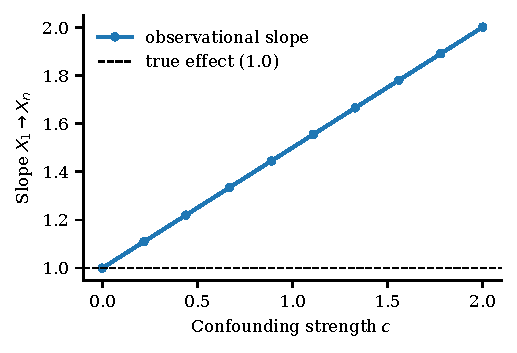
\includegraphics[width=\columnwidth]{figs/fig03_causal.pdf}
\caption{Observational slope from $X_1$ to $X_n$ versus confounding strength (pilot, linear SCM). Dashed line: true causal effect.}
\label{fig:fig03_causal}
\end{figure}

\section{Discussion and Limitations}
The simulated graphs are the ground truth, so the study does not establish causality in real systems. Text-extracted statements may be noisy, and the protocol reports results both with clean and with corrupted statements.

\section{Conclusion}
The proposed protocol separates correlation-based prediction from interventional consistency in a setting where the true answer is known, and tests whether text-derived causal statements help.

\section*{Acknowledgments}
The author thanks the Brazilian artificial intelligence community.

\nocite{ctl_full_names}
\bibliographystyle{IEEEtran}
\bibliography{refs}

\end{document}
